\chapter{Physical Backgrounds}
\label{chap:bkgs}
\chapquote{Today's prediction is tomorrow's prior.}{Glen Cowan, during TAE summer school 2017}
Regarding G.~Cowan's quote about tomorrow's prior, decays that were first observed during \gls{runone}, such as $\decay{\Lb}{\Lz\Ph\Ph'}$ and \decay{\Bsb}{\Dz\KS} not only have become today's prior, they already have to be considered as background candidates in \gls{runtwo} analyses.
In this section we discuss those and other physical background contributions which we separate into non-resonant backgrounds (Sec.~\ref{sec:bkgs_nonres}), partially reconstructed backgrounds (Sec.~\ref{sec:bkgs_part}), and \glspl{reflection} (Sec.~\ref{sec:bkgs_refl}).
While we find that most background contributions can be neglected due to a sufficiently strong suppression, partially reconstructed decays including \Dstarz resonances or \Sz baryons, stay a nuisance and enter the fit model of the subsequent $m(\Dz\Lz)$ fit.

\section{Non-Resonant Background}
\label{sec:bkgs_nonres}
\decay{\Lb}{\Dz\proton\pim} decays have the potential of being a dangerous (non-resonant) background for the \decay{\Lb}{\Dz\Lz} mode, if the \Lz daughters are reconstructed as \gls{LL} tracks.
If not sufficiently suppressed, this background is irreducible in the $m(\Dz\Lz)$ distribution and very hard to unfold from genuine \decay{\Lb}{\Dz\Lz} decays by conventional fitting approaches.
Luckily for the present analysis, the kinematic suppression of the \gls{stripping} phase already gives a strong suppression,\footnote{Mostly due to the required finite mass window around $m(\Lz)$.} as shown in Chap.~\ref{chap:stripeff}.
Applying the dedicated tight \decay{\Lb}{\Dz\Lz} selection (\cf{}~Sec.~\ref{sec:LbToDzLz_tightsel}) gives an additional suppression and accepts \num{65} of \num{46740} (weighted) events, where the latter is the amount of events that already pass the dedicated pre- and loose \decay{\Lb}{\Dz\Lz} selection steps.\footnote{Technically, we use so-called \textit{filtered} events for this task. Filtered events give larger yields but estimating the combined reconstruction and \gls{stripping} efficiency is more challenging than for ordinary simulated events (which we used for the latter task).}
A 95\,\% confidence interval of the corresponding efficiency is $[1.1 \ldots 1.8]\,\times 10^{-3}$.
The efficiencies of each selection step individually, without requiring any of the other criteria, are shown in Tab.~\ref{tab:LbToDzppi_bkg_tightseleffs}.
\begin{table}[htbp]
    \centering
    \caption{Efficiencies of applying the tight selection criteria as found in Sec.~\ref{sec:LbToDzLz_tightsel} of the \decay{\Lb}{\Dz\Lz} selection to genuine \decay{\Lb}{\Dz\proton\pim} decays, evaluated with \gls{mc} simulated events.}
    \label{tab:LbToDzppi_bkg_tightseleffs}
    \begin{tabular}{lS[separate-uncertainty=false]}
        \toprule
        Selection criterion & {Efficiency [\%]} \\
        \midrule
        \Lz Clf. $\ge 0.67$ & 4.68 \pm 0.10 \\
        \Lb-\Dz Clf. $\ge 0.73$ & 19.26 \pm 0.18 \\
        \texttt{ProbNNp} $\ge 0.6$ & 22.87 \pm 0.19 \\
        \texttt{ProbNNk} $\ge 0.3$ & 23.35 \pm 0.20 \\
        \Gls{dtf} prob. $\ge 0.012$ & 0.61 \pm 0.04 \\
        \midrule
        Combination & 0.139 \pm 0.017 \\
        \bottomrule
    \end{tabular}
\end{table}
Combining this efficiency with the suppression factor of the \gls{stripping} phase leverages the estimation of an upper limit of the accumulated probability $P$ of seeing at most $n$ genuine \decay{\Lb}{\Dz\proton\pim} events in the invariant mass of \Dz and \Lz candidates:
\begin{equation*}
    P = \sum_{k=0}^n \begin{pmatrix} N \\ k \end{pmatrix} p^k (1-p)^{N-k} \,.
\end{equation*}
In Fig.~\ref{fig:LbToDzppi_bkg_efflimit} we show the accumulated probability for $p=9 \times 10^{-5}$ (dashed line) which corresponds to a conservative approximation of both factors.
\begin{figure}[htbp]
    \centering
    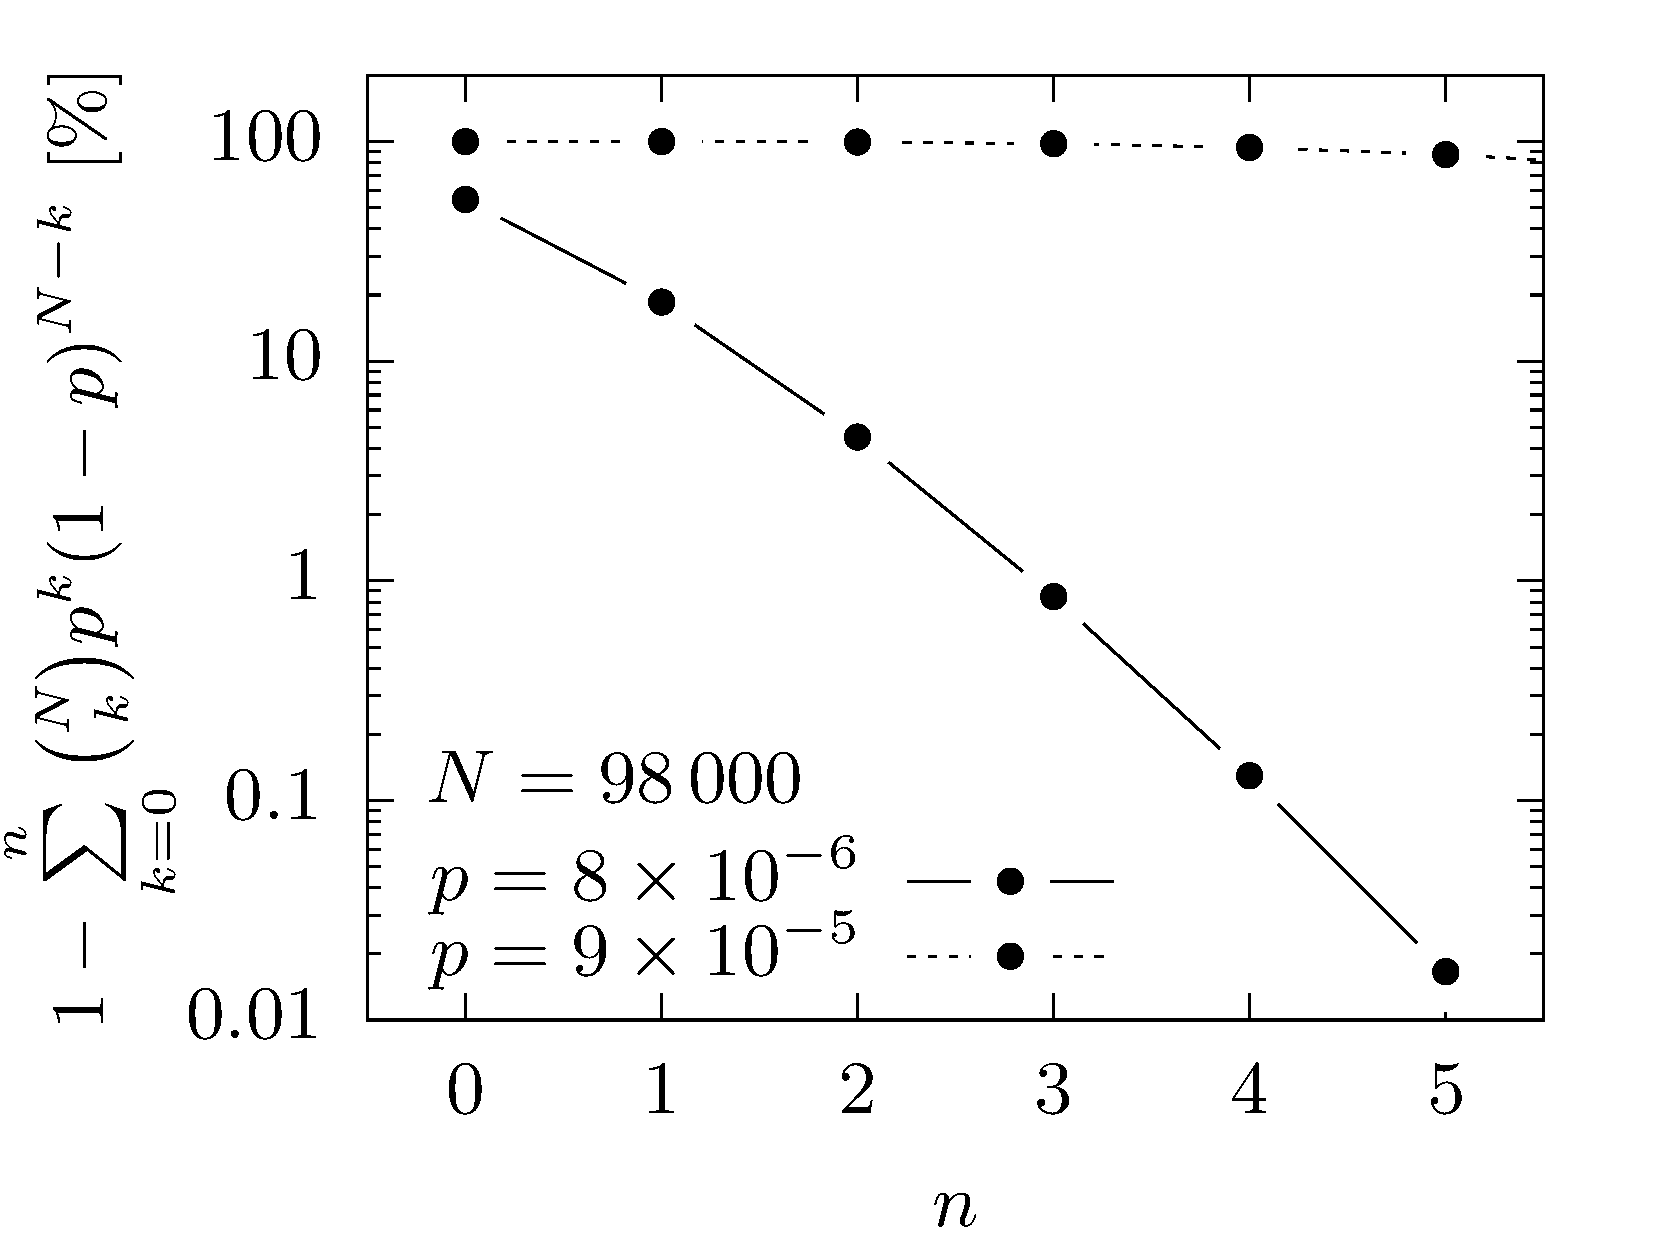
\includegraphics[scale=1.]{Lb2Dzppi_bkg/binom_prob_acc.png}
    \caption{Probability of seeing more than $n$ genuine \decay{\Lb}{\Dz\proton\pim} decays in $m(\Dz\Lz)$. The solid (dashed) line corresponds to our choice of selection steps, including (excluding) the additional selection requirements w.r.t.\ $m(\proton\pim)$ and the \Lz flight distance significance.}
    \label{fig:LbToDzppi_bkg_efflimit}
\end{figure}
We argue that this suppression on its own is not sufficient.
In the following we will therefore tighten the mass window of $m(\proton\pim)$ around $m(\Lz)$ and establish a veto against small values of the \Lz flight distance significance.
These additional requirements decrease the combined efficiency to at most $p=8 \times 10^{-6}$ at a 95\,\% CL (solid line in Fig.~\ref{fig:LbToDzppi_bkg_efflimit}), corresponding to a probability of seeing not more than three events above $99\,\%$.

\begin{figure}[htbp]
    \centering
    \begin{subfigure}{.49\textwidth}
        \centering
        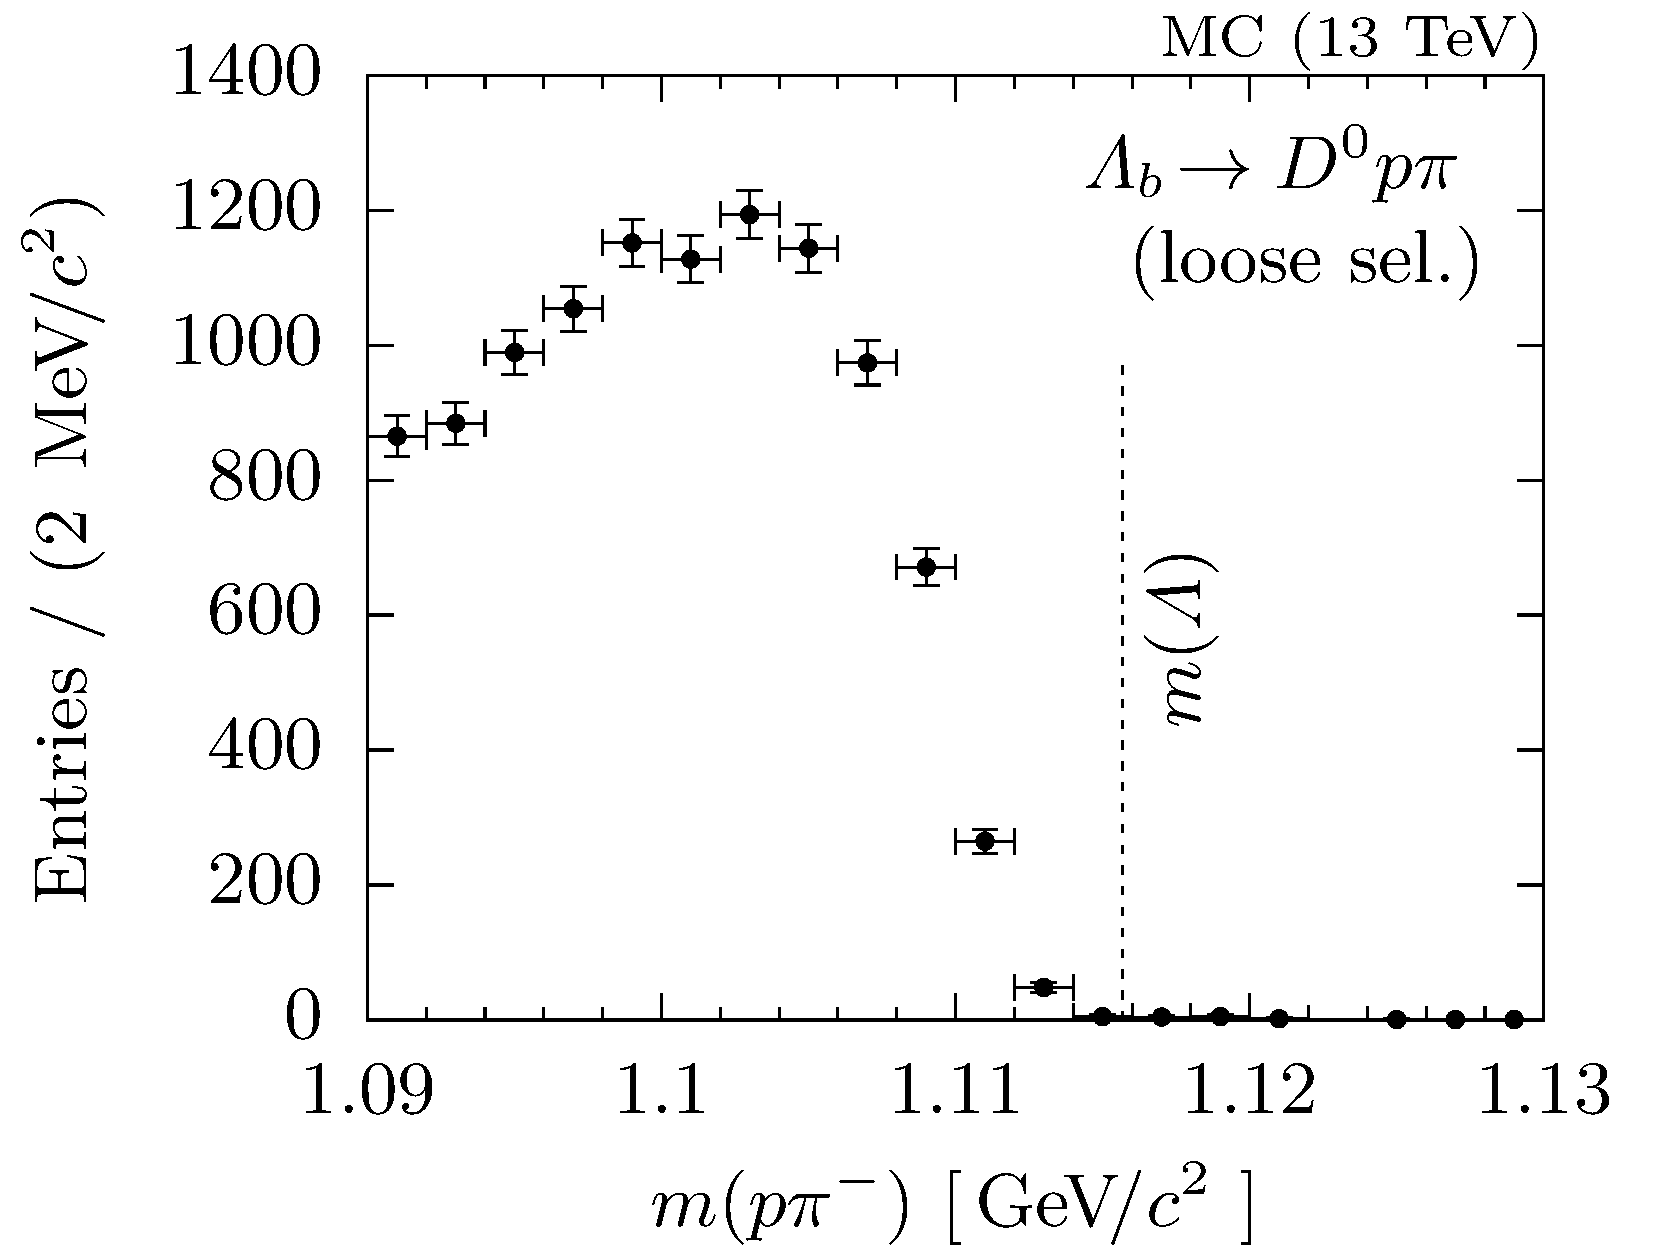
\includegraphics[scale=1.]{Lb2Dzppi_bkg/mLz_loose.png}
    \end{subfigure}
    \begin{subfigure}{.49\textwidth}
        \centering
        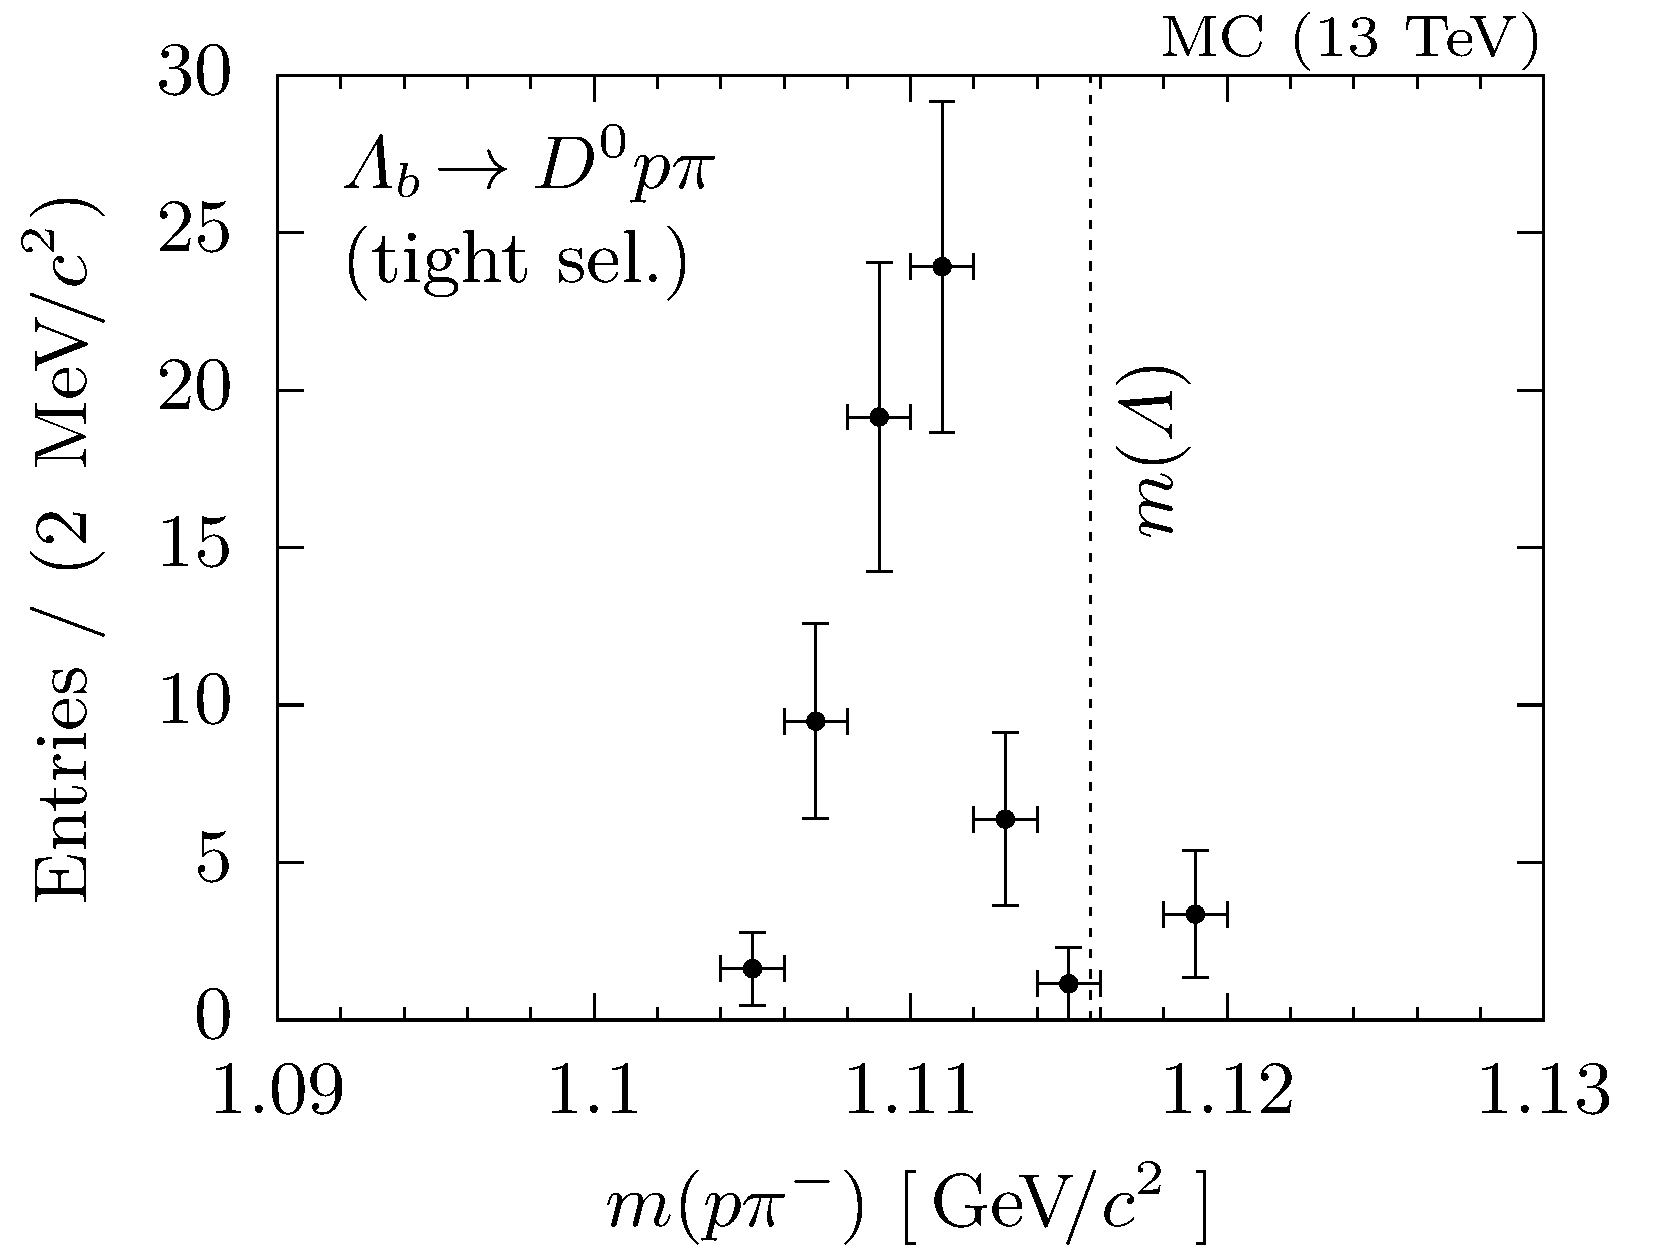
\includegraphics[scale=1.]{Lb2Dzppi_bkg/mLz.png}
    \end{subfigure}
    \caption{Combined invariant mass of \proton and \pim candidates of simulated \decay{\Lb}{\Dz\proton\pim} decays, reconstructed and fitted via a \gls{dtf} as \decay{\Lb}{\Dz\Lz}. The loose selection (left) and tight selection (right) are the dedicated \decay{\Lb}{\Dz\Lz} selections as described in Sec.~\ref{sec:LbToDzLz_prepro}.}
    \label{fig:LbToDzppi_bkg/mLz}
\end{figure}
In Fig.~\ref{fig:LbToDzppi_bkg/mLz} we show the invariant mass distribution of $m(\proton\pim)$ before and after applying the dedicated \decay{\Lb}{\Dz\Lz} tight selection.
Apparently, it is not flat but strongly (asymmetrically) suppressed for $m(\proton\pim)>m(\Lz)$.
We find that this structure is introduced by requiring a minimum flight distance (\cf{}~Sec.~\ref{sec:LbToDzLz_loosesel}) and simultaneously constraining the \Lz mass in a \gls{dtf} (\cf{} Appx.~\ref{chap:apdx_dtf} for a more detailed description of this correlation.)
We choose
\begin{align*}
    m(\proton\pim) - m(\Lz_\text{PDG}) &\overset{!}{>} -4\mev \,, \\
    \text{\Lz FD sig.} &\overset{!}{>} 25 \,,
\end{align*}
where $m(\Lz_\text{PDG})$ is taken from Ref.~\cite{pdg},
as thresholds for $m(\proton\pim)$ and the flight distance significance of the \Lz baryon which leaves, when applied in combination, only one event left (weight $1.12$).
In Fig.~\ref{fig:Lb2Dzppi_bkg_fdsig_cdf} we show the cumulative distribution of the latter in combination with and without the tight selection.
With $n<2$ and a preselection suppression factor of $20$ this corresponds to an 95\,\% confidence interval of $[0.26 \ldots 8]\,\times 10^{-6}$.
\begin{figure}[htbp]
    \centering
    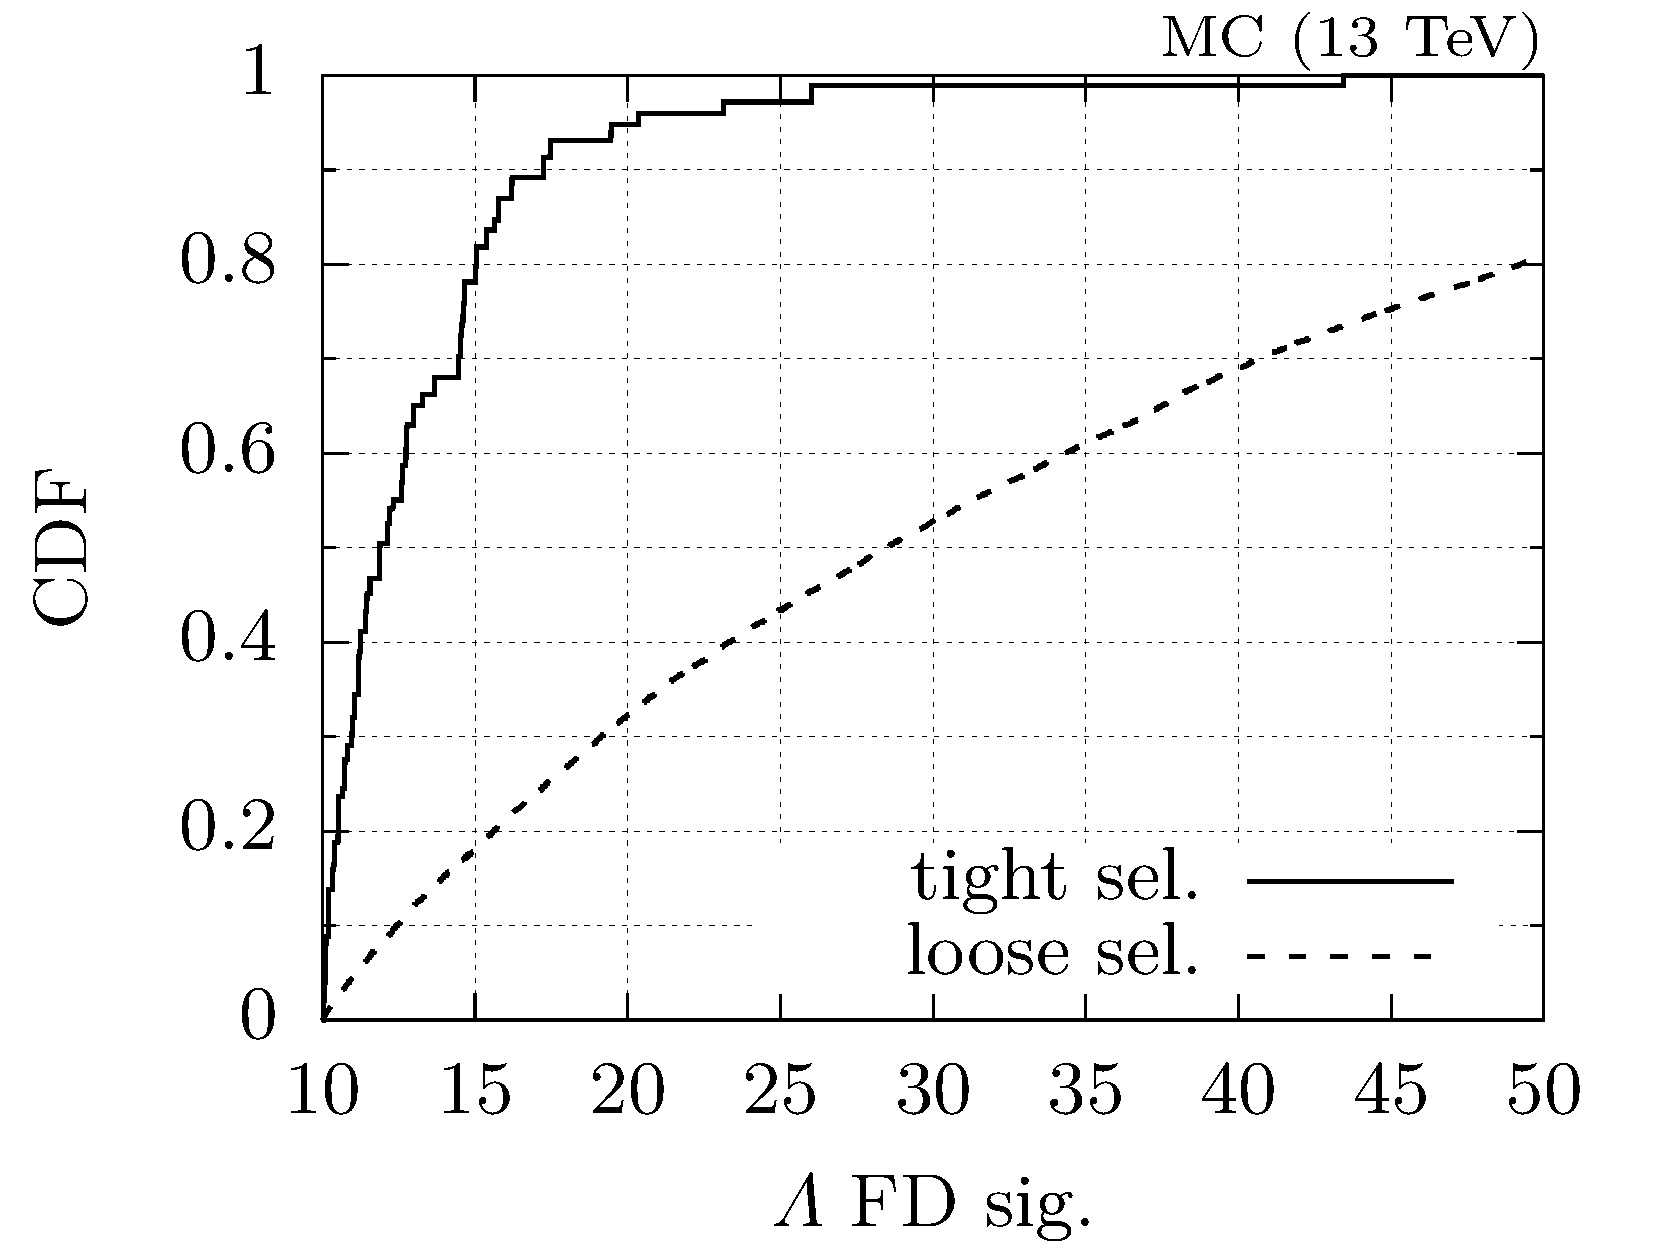
\includegraphics[scale=1.]{Lb2Dzppi_bkg/fdsig_cdf.png}
    \caption{Cumulative distribution of selections w.r.t.\ the flight distance significance of the (spurious) \Lz candidates from \decay{\Lb}{\Dz\proton\pim} decays after (solid line) and before (dashed line) applying the dedicated tight \decay{\Lb}{\Dz\Lz} selection.}
    \label{fig:Lb2Dzppi_bkg_fdsig_cdf}
\end{figure}

We refer to Ref.~\cite{LbToDzphAndLch} for studies of Dalitz plots of \decay{\Lb}{\Dz\proton\pim} decays and note that the \Lz baryon is located at low values of $m^2_{\proton\pion}$ and large values of $m^2_{\PD\proton}$.
Both areas show no large resonance structures and thus support the conservative trait of our approximation.

\section{Partially Reconstructed Backgrounds}
\label{sec:bkgs_part}
In the present analysis partially reconstructed backgrounds come from intermediate states that decay to either a soft photon or a soft neutral pion.
These low energetic particles typically escape undetected at \lhcb and thus making the respective backgrounds irreducible.
In particular, we will consider \decay{\Lb/\Xibz}{\Dz\Sz} and \decay{\Xibz}{\Dz\Xiz} decays, as well as \decay{\Lb/\Xibz}{\Dstarz\Lz}, where in the former cases the \Pgamma (\piz) from \decay{\Sz}{\Lz\Pgamma} (\decay{\Xiz}{\Lz\piz}), and in the latter case the \Pgamma (\piz) from \decay{\Dstarz}{\Dz\Pgamma} (\decay{\Dstarz}{\Dz\piz}) is lost.
We devoted the entire Sec.~\ref{sec:isospin} of our theory part to the discussion of the irreducible \decay{\Sz}{\Lz\Pgamma} background.
In addition we analyze its kinematics, as well as the kinematics of the other partially reconstructed background sources in depth in Appx.~\ref{chap:apdx_partbkg}.
Since these backgrounds are irreducible we will encounter them in our fitting model.

\section{Reflections}
\label{sec:bkgs_refl}
Apart from random track combinations, non-resonant and partially reconstructed decays, so-called \textit{\glspl{reflection}} potentially contaminate the signal region in the invariant mass distribution $m(\Dz\Lz)$.
\Glspl{reflection} are fully reconstructed decays where a spurious mass hypothesis was assigned to at least one of the particles within the respective decay chain.
Since reconstruction is typically performed in the upstream direction of the respective decay chain, this wrong assignment also propagates as a shift and dilution of the mass distributions.
Decays, such as \decay{\Bsb}{\Dz\KS}, can contaminate the signal region if the kaon decay \decay{\KS}{\pip\pim} becomes a \gls{reflection} by misidentifying the \pip as a proton and thus fakes a \decay{\Lz}{\proton\pim} decay.
This smears the invariant mass distribution of the \KS, as well as the \Bs meson mass distribution and consequently introduces background contributions to the invariant mass distribution $m(\Dz\Lz)$.

For a given $n$-body decay the invariant mass of the mother $M$ is given by the invariant masses $m_i$ and three-momenta $\vec{p}_i$ of the daughters via the relation
\begin{equation*}
    M^2 = \left( \sum_{i=1}^n \sqrt{m_i^2 + \vec{p}_i^{\,2}} \right)^2 - \left( \sum_{i=1}^n \vec{p}_i \right)^2 \,.
\end{equation*}
The shift of $M$ in case of a spurious mass hypothesis $m_j \to m_j + \delta m_j$ is non-linear in $\delta m_j$ and depends on the respective momenta, hence the transformation of the invariant mass distributions due to \glspl{reflection} is non-trivial and depend on the momentum distributions.

In the following we discuss the two main sources of \glspl{reflection} in the present analysis.
In Sec.~\ref{sec:bkgs_charmless} we study charmless three-body decays and then discuss the possible contamination of genuine \KS decays in Sec.~\ref{sec:bkgs_ks}.
Both background candidates are eventually found to be negligible given the amount of available statistics after applying the dedicated tight \decay{\Lb}{\Dz\Lz} selection and are thus not included in the subsequent $m(\Dz\Lz)$ fit model.

\subsection{Charmless Decays}
\label{sec:bkgs_charmless}
Charmless three-body decays $\decay{\Lb/\Xibz}{\Lz\Ph\Ph'}$ are a nuisance in searches for \CP violation in \decay{\Lb}{\Dz\Lz} decays when $\Ph\Ph'$ are spuriously reconstructed as $\decay{\Dz}{\Ph\Ph'}$.
The reported branching fractions are (\cf{}~Refs.~\cite{pdg,LbToLzhh})
\begin{align*}
    \BR(\decay{\Lb}{\Lz\Kp\Km}) &= (1.62 \pm 0.23) \times 10^{-5} \,, \\
    \BR(\decay{\Lb}{\Lz\Kp\pim}) &= (5.7 \pm 1.3) \times 10^{-6} \,, \\
    \BR(\decay{\Lb}{\Lz\pip\pim}) &= (4.7 \pm 1.9) \times 10^{-6} \,, 
\end{align*}
and thus will appear as physical background in the relevant \gls{ads} and \gls{glw} modes.
Similarly, \decay{\Xibz}{\Lz\Kp\Km}, \decay{\Xibz}{\Lz\Km\pip} and \decay{\Xibz}{\pip\pim} decays are background candidates in \decay{\Xibz}{\Dz\Lz} analyses.
All these modes are hard to control and require decent statistics to, for example, estimate their contribution to the signal yields by analyzing the combined invariant masses of \Dz and \Lz candidates in slices of the \Dz flight distance.
Beneficially for the present analysis, the \decay{\Lb}{\Lz\Km\pip} decay is suppressed w.r.t.\ \decay{\Lb}{\Lz\Kp\pim} with at least a factor of a box diagram and neither \decay{\Lb}{\Lz\Km\pip}, nor \decay{\Xibz}{\Lz\Km\pip} were observed experimentally at the time of writing.

For the present analysis where we reconstruct the \Dz meson as \decay{\Dz}{\Km\pip}, the \decay{\Lb}{\Lz\Kp\Km} background only enters indirectly via \gls{reflection}.
Below, we show that we can suppress the contribution coming from \decay{\Lb}{\Lz\Kp\Km} decays (largest branching fraction) sufficiently and thus renders dedicated analyses of the remaining \decay{\Lb}{\Lz\Ph\Ph'} modes unnecessary.
We use weighted, \gls{truthmatched} \gls{mc} simulated events\footnote{Generated flat in phase space.} for this task where we rely on the established weights without adding acceptance corrections due to the limited dataset.

First, we apply the dedicated \decay{\Lb}{\Dz\Lz} preselection step with the tightened requirements we established in Sec.~\ref{sec:bkgs_nonres} which already greatly reduces the \decay{\Lb}{\Lz\Kp\Km} data set from \num{2875} to \num{570} and \num{7055} to \num{1785} events\footnote{The reduced numbers are the accumulated weights of the \gls{mc} simulated events.} for \gls{LL} and \gls{DD} tracks, respectively.\footnote{This strong suppression is driven by the fact that the dedicated \decay{\Lb}{\Dz\Lz} preselection step already includes requirements w.r.t.\ the fit probability, \Dz flight distance, etc.}
Secondly, we apply the selection steps w.r.t.\ the \gls{dtf} probability, and the responses of the \texttt{ProbNNp} and \texttt{ProbNNk} classifiers for the \proton and \Km, respectively.
The corresponding efficiencies are listed in Tab.~\ref{tab:bkgs_charmless_nonclfeff}.
The efficiencies for the selection requirements w.r.t.\ \texttt{ProbNNp} and \texttt{ProbNNk} are compatible with those we found for genuine \decay{\Lb}{\Dz\Lz} decays, whereas the \gls{dtf} reveals its strong separation power due to the \Dz mass constraint.
\begin{table}[htbp]
    \centering
    \caption{Efficiencies of the dedicated \decay{\Lb}{\Dz\Lz} tight selection requirements when applied to \decay{\Lb}{\Lz\Kp\Km}, reconstructed as \decay{\Lb}{\Dz\Lz}, and genuine \decay{\Lb}{\Dz\Lz} decays. The efficiencies are obtained from weighted \gls{mc} simulated events.}
    \label{tab:bkgs_charmless_nonclfeff}
    \begin{tabular}{l%
                    S[separate-uncertainty=false,table-format=2.2(2)]%
                    S[separate-uncertainty=false,table-format=2.2(2)]%
                    S[separate-uncertainty=false,table-format=2.2(2)]%
                    S[separate-uncertainty=false,table-format=2.2(2)]}
        \toprule
        & \multicolumn{2}{c}{{\decay{\Lb}{\Lz\Kp\Km}}} & \multicolumn{2}{c}{{\decay{\Lb}{\Dz\Lz}}} \\
        & {\gls{LL} [\%]} & {\gls{DD} [\%]} & {\gls{LL} [\%]} & {\gls{DD} [\%]} \\
        \midrule
        \Gls{dtf} prob. & 43.5 \pm 2.1 & 28.1 \pm 1.1 & 89.16 \pm 0.31 & 82.07 \pm 0.24 \\
        $\texttt{ProbNNp}(\proton)$ & 94.2 \pm 1.0 & 86.6 \pm 0.8 & 92.87 \pm 0.26 & 81.54 \pm 0.25 \\
        $\texttt{ProbNNk}(\kaon)$ & 91.3 \pm 1.2 & 84.7 \pm 0.9 & 92.51 \pm 0.26 & 84.50 \pm 0.23 \\
        \midrule
        Combination & 26.4 \pm 1.8 & 24.9 \pm 1.0 & 88.51 \pm 0.32 & 88.67 \pm 0.20 \\
        \bottomrule 
    \end{tabular}
\end{table}

The efficiencies of applying the \Lz and \Lb-\Dz classifier selection requirements are estimated after applying all previous discussed selections and are listed in Tab.~\ref{tab:bkg_charmless_clfeff}.
Interestingly, both classifiers show a strong separation power, except for the \Lz classifier when applied to \gls{LL} tracks.
In order to understand this behavior we train \glspl{svm} on the reduced data set using all pairwise combinations of two features to estimate each feature importance.
For the \Lb-\Dz classifier we find that almost the entire separation power stems from the \Dz flight distance feature.
This is expected, since in the case of genuine \decay{\Lb}{\Lz\Kp\Km} decays, the fitted flight distance of the \Kp\Km pair is smaller on average than for genuine \Dz meson.
More surprisingly, the \Lz classifier is also capable to separate between genuine \decay{\Lb}{\Dz\Lz} and \decay{\Lb}{\Lz\Kp\Km} decays.
The rather large deviation for \gls{LL} and \gls{DD} tracks is rooted in the mild thresholds of the former but adjusts when the thresholds are raised.
Using the same technique we used previously, we find that the separation power is driven by deviations in the \pt distributions which we discuss in detail in Appx.~\ref{sec:apdx_charmlessrel_Lzp}.
\begin{table}[htbp]
    \centering
    \caption{Efficiencies of the optimized \decay{\Lb}{\Dz\Lz} tight selection requirements when applied to \decay{\Lb}{\Lz\Kp\Km}, reconstructed as \decay{\Lb}{\Dz\Lz}, and genuine \decay{\Lb}{\Dz\Lz} decays. The efficiencies are obtained from weighted \gls{mc} simulated events after applying the selection steps listed in Tab.~\ref{tab:bkgs_charmless_nonclfeff}.}
    \label{tab:bkg_charmless_clfeff}
    \begin{tabular}{l%
                    S[separate-uncertainty=false,table-format=2.2(2)]%
                    S[separate-uncertainty=false,table-format=2.2(2)]%
                    S[separate-uncertainty=false,table-format=2.2(2)]%
                    S[separate-uncertainty=false,table-format=2.2(2)]}
        \toprule
        & \multicolumn{2}{c}{{\decay{\Lb}{\Lz\Kp\Km}}} & \multicolumn{2}{c}{{\decay{\Lb}{\Dz\Lz}}} \\
        & {\gls{LL} [\%]} & {\gls{DD} [\%]} & {\gls{LL} [\%]} & {\gls{DD} [\%]} \\
        \midrule
        \Lz Clf. & 97.5 \pm 1.1 & 34.3 \pm 2.7 & 96.54 \pm 0.21 & 50.3 \pm 0.4 \\
        \Lb-\Dz Clf. & 68 \pm 4 & 31.0 \pm 2.6 & 80.0 \pm 0.5 & 47.0 \pm 0.4 \\
        \midrule
        Combination & 67 \pm 4 & 18.9 \pm 2.1 & 77.9 \pm 0.5 & 33.5 \pm 0.4 \\
        \bottomrule 
    \end{tabular}
\end{table}

Applying the entire dedicated \decay{\Lb}{\Dz\Lz} tight selection leaves 122 and 72 weighted events left for \gls{LL} and \gls{DD} tracks, respectively.
Their corresponding invariant mass distributions $m(\Dz\Lz)$ are shown in Fig.~\ref{fig:LbToLzKK_bkg_hLbM}. (We refer to Appx.~\ref{sec:apdx_charmlessrefl_mass} for a brief discussion of these mass distributions.)
Using the suppression factor for \gls{LL} and \gls{DD} tracks that we established in Sec.~\ref{chap:stripeff}, we expect $7.8(15)$ and $4.8(9)$ genuine \decay{\Lb}{\Lz\Kp\Km} events after the dedicated \decay{\Lb}{\Dz\Lz} tight selection steps.
\begin{figure}[htbp]
    \centering
    \begin{subfigure}{.49\textwidth}
        \centering
        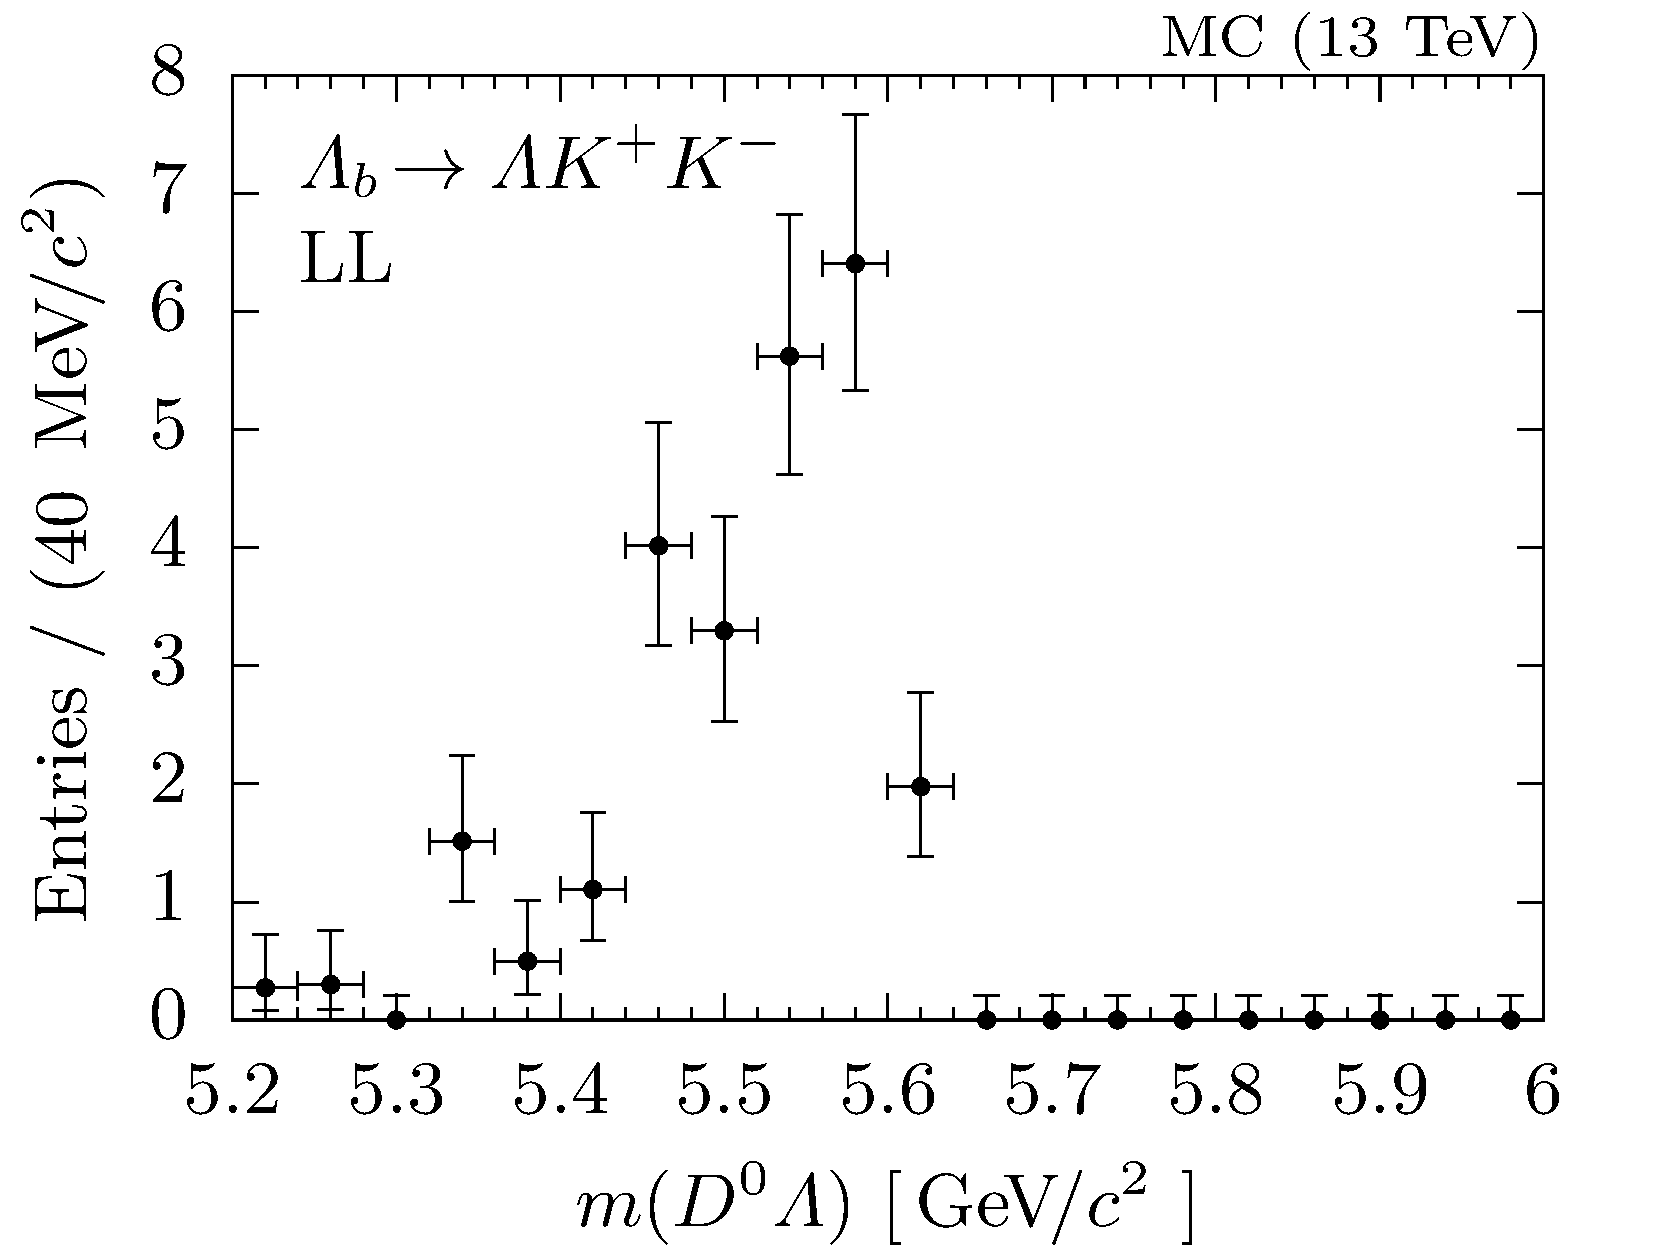
\includegraphics[scale=1.]{Lb2LzKK_bkg/hLbM_LL.png}
    \end{subfigure}
    \begin{subfigure}{.49\textwidth}
        \centering
        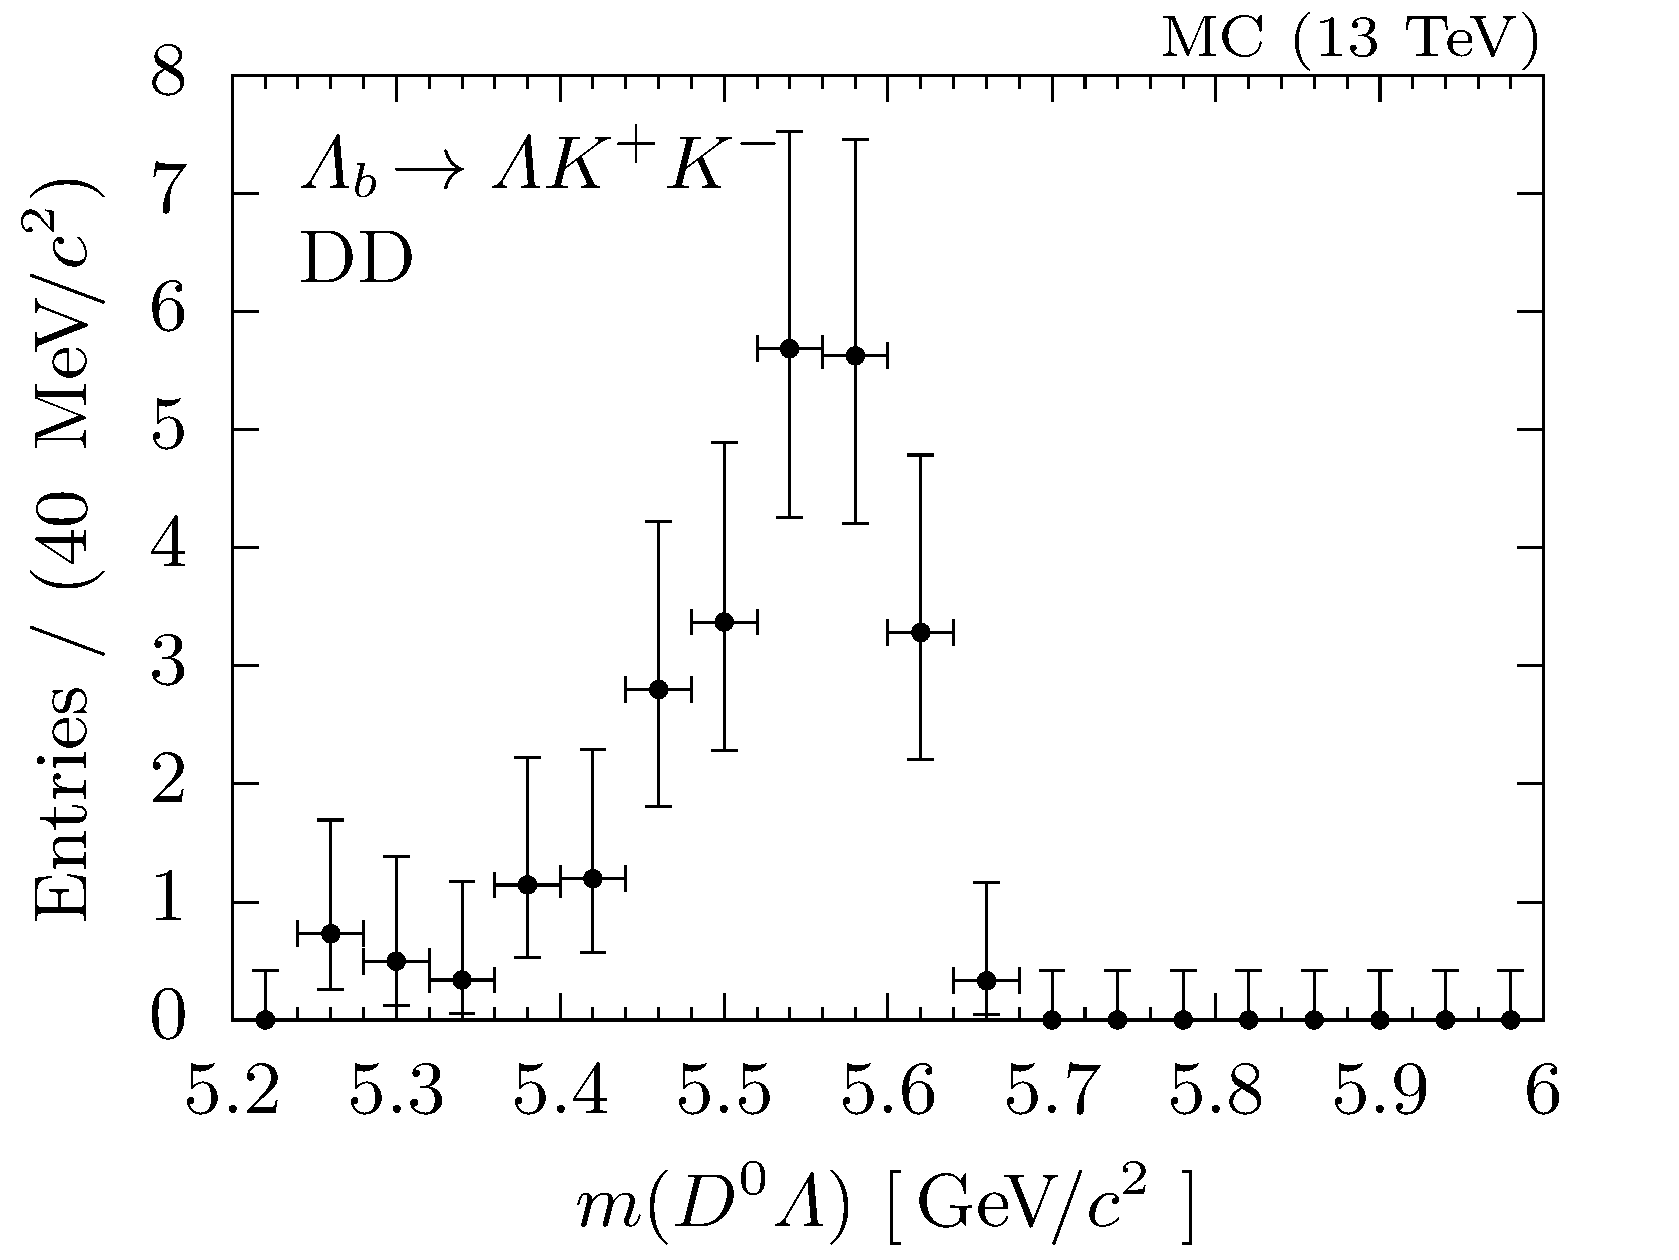
\includegraphics[scale=1.]{Lb2LzKK_bkg/hLbM_DD.png}
    \end{subfigure}
    \caption{Combined invariant mass of \decay{\Dz}{\Km\pip} and \decay{\Lz}{\proton\pim} candidates from \gls{mc} simulated \decay{\Lb}{\Lz\Km\Kp} decays for \gls{LL} (left) and \gls{DD} (right) tracks.}
    \label{fig:LbToLzKK_bkg_hLbM}
\end{figure}

In theory, these amounts could be suppressed further by requiring a minimal flight distance of the \Dz candidates.
For example, requiring
\begin{equation}
    \label{eq:bkgs_dzfdsigreq}
    \text{\Dz FD sig.} > 2 \,,
\end{equation}
reduces the expectation of genuine \decay{\Lb}{\Lz\Kp\Km} events to $2.6(6)$ and $0.79(26)$, but also suppresses \decay{\Lb}{\Dz\Lz} to $83.6(5)\,\%$ and $80.7(5)\,\%$ for \gls{LL} and \gls{DD}, respectively (\cf{}~Fig.~\ref{fig:apdx_charmlessrel_fdDz}).
Alternatively, the reflection shape can be parametrized and fitted in recorded data.
However, regarding the limited data sample, we find in Chap.~\ref{chap:fit} that an unfolding from \decay{\Xibz}{\Dstarz\Lz} contributions is not possible and since the latter component is disfavored by our fit model, we argue that \decay{\Lb}{\Lz\Kp\Km} contributions in the signal region are negligible without further suppression.
We cross-check this assumption by requiring Eq.~\eqref{eq:bkgs_dzfdsigreq} and fitting the invariant mass of \Dz and \Lz candidates from recorded data in configuration 1.
(See Chap.~\ref{chap:fit} for a description of the fit model and its configurations, as well as Fig.~\ref{fig:fit_hLbM_dsig2} for a projection of the fit to recorded data.)
The fitted signal yield of \decay{\Lb}{\Dz\Lz} decays reduces from $31(7)$ to $23(6)$.
Assuming a reduction of $82\,\%$ (combination of both track types), the expected yield is $25.4(21)$ and thus includes the fitted yield within two standard deviations.
We thus conclude that \decay{\Lb}{\Lz\Kp\Km} events contribute negligible in the signal region.
Since \decay{\Xibz}{\Lz\Km\pip} decays are expected to behave similarly and due to the additional \gls{ckm} suppression w.r.t.\ \decay{\Xibz}{\Dz\Lz} decays, we argue further that the contribution of charmless backgrounds in the \Xibz mode is negligible, too.

\subsection{\texorpdfstring{\KS}{Neutral Kaon} Reflections from \texorpdfstring{\bquark}{b}-Meson Decays}
\label{sec:bkgs_ks}
In the decay \decay{\Lb}{\Dz\Lz} we expect \glspl{reflection} coming from \Bd and \Bs meson decays to \Dz\KS, caused by a misidentification of the \pip in \decay{\KS}{\pip\pim}.
The leading contribution to the decays \decay{\Bdb}{\Dz\KS} and \decay{\Bsb}{\Dz\KS} are internal, color-suppressed tree diagrams, where the former includes the Cabibbo suppressed \decay{\bquark}{\cquark\squark\uquarkbar} transition and the latter the Cabibbo favored \decay{\bquark}{\cquark\dquark\uquarkbar} transition.
The respective \Bd branching fraction is well established, measured by the \gls{babar} and \gls{belle} collaborations~\cite{BdToDK1,BdToDK2}, and the \Bs mode was first observed and measured at \lhcb~\cite{BsToDK}:
\begin{align*}
    \mathcal{B}(\decay{\Bdb}{\Dz\Kzb}) &= (5.2 \pm 0.7) \times 10^{-5} \,,\\
    \mathcal{B}(\decay{\Bsb}{\Dz\Kz}) &= (4.3 \pm 0.9) \times 10^{-4} \,.
\end{align*}
Besides being very useful for leveraging access to the \gls{ckm} phase $\gamma$ and even $\phi_\squark$ in the latter case, both branching fractions are significantly larger than the expected branching fraction of \decay{\Lb}{\Dz\Lz}~\cite{brLbToDzLz_pred},
%\begin{equation}
%    \label{eq:bkgs_LbToDzLz_pred}
%    \mathcal{B}(\Lb \to D^0 \Lz) = 4.56 \times 10^{-6} \,,
%\end{equation}
making them also background candidates for the present analysis.
However, it is the fraction $\kappa$ of misidentified \Bd and \Bs mesons in the signal region of \decay{\Lb}{\Dz\Lz} that has to be considered.
This fraction can be estimated by the product of ratios of the \bquark-hadron productions (I), the branching fractions of the respective decay modes (II), the reconstruction efficiencies (III), and the selection efficiencies (IV):
\begin{multline*}
    \kappa(\PB^0_{(\squark)}) := \underbrace{\frac{f_{\PB^0_{(\squark)}}}{f_{\Lb}}}_{\text{I}} \times \underbrace{\frac{\mathcal{B}(\decay{\Bbar{}^0_{(\squark)}}{\Dz\KS})}{\mathcal{B}(\decay{\Lb}{\Dz\Lz})} \times \frac{\mathcal{B}(\decay{\KS}{\pip\pim})}{\mathcal{B}(\decay{\Lz}{\proton\pim})}}_{\text{II}} \\
    \times \underbrace{\frac{\varepsilon_\text{rec}(\decay{\Bbar{}^0_{(\squark)}}{\Dz\KS})}{\varepsilon_\text{rec}(\decay{\Lb}{\Dz\Lz})}}_{\text{III}} \times \underbrace{\frac{\varepsilon_\text{sel}(\decay{\Bbar{}^0_{(\squark)}}{\Dz\KS})}{\varepsilon_\text{sel}(\decay{\Lb}{\Dz\Lz})}}_{\text{IV}}.
\end{multline*}
%The objective of the this section is to minimize $\kappa$ by tuning factor IV.
The relative production rates (I) are measured by \lhcb~\cite{LHCb_bProdFrac_7,LHCb_bProdFrac_13}.
Factor II is found by inserting the theory prediction from Ref.~\cite{brLbToDzLz_pred} and the respective established branching ratios,\footnote{The kaon in the decay of the \Bd (\Bs) meson is produced in an unmixed flavor eigenstate \Kzb (\Kz), whereas the time-evolution propagates the mass eigenstates \KL and \KS. Here, we assume $|\langle \KS | \Kz \rangle|^2 = |\langle \KS | \Kzb \rangle|^2 = 1/2$ and thus neglecting \CP{} violating effects in the kaon system which are known to be at a level of $10^{-3}$~\cite{pdg}.}:
\begin{equation*}
    \frac{\mathcal{B}(\decay{\Bbar{}^0_{(\squark)}}{\Dz\KS})}{\mathcal{B}(\decay{\Lb}{\Dz\Lz})} \times \frac{\mathcal{B}(\decay{\KS}{\pip\pim})}{\mathcal{B}(\decay{\Lz}{\proton\pim})} =
    \begin{cases}
        6.2(8) & \text{for } \decay{\Bdb}{\Dz\KS} \,, \\
        51(11) & \text{for } \decay{\Bsb}{\Dz\KS} \,.
    \end{cases}
\end{equation*}
The final approximation will be dominated by the vague uncertainty of the theory prediction for $\mathcal{B}(\decay{\Lb}{\Dz\Lz})$, hence we aim for an upper limit of $\kappa$.
In this context we assume the ratio of the reconstruction efficiencies (III) to be one in good approximation.
Factor IV for \decay{\Bsb}{\Dz\KS} is found using weighted simulated events and used as an upper limit of \decay{\Bdb}{\Dz\KS}.
Due to the lack of a sufficient amount of \gls{mc} simulated events we use the simulation framework \texttt{RapidSim}~\cite{rapidsim} instead.
These simulated events are calibrated with weights obtained from \decay{\Bd}{\jpsi\KS} rather than \decay{\Lb}{\jpsi\Lz} decays due to the initial \bquark-meson, using the same techniques outlined in Sec.~\ref{sec:LbToJpsiLz_w1}.
Similar to the previous sections,\footnote{For the sake of brevity we abstain from a detailed discussion. The chosen techniques are equivalent to the ones that were outlined previously, and the remarkable strong suppression of rectangular selections w.r.t.\ mass and \texttt{ProbNNp} tolerate large uncertainties. \texttt{RapidSim}'s fidelity issues concerning the resolution of \KS particles is found to be negligible in this context.} we find a sufficient suppression, due to the very broad $m(\proton\pim)$ distribution for misidentified \decay{\KS}{\pip\pim} decays, on its own allowing a suppression (factor IV) below $3\,\%$ without loosing any genuine \decay{\Lz}{\proton\pim} event.
Applying the entire \decay{\Lb}{\Dz\Lz} tight selection eventually reduces $\kappa(\Bsb)$ below $4\,\%$ at a 95\,\% confidence level, rendering an additional suppression, \eg{}, via a $m(\Kz)$ veto unnecessary.
